\chapter{Optimal Transport for Dynamical Systems}
\label{cha:theory_background}

\dictum[Elinor Ostrom, \textit{Governing the Commons} (1990)]{%
  The power of a theory is exactly proportional to the diversity of situations it can explain.}%
\vskip 2em


Optimal transport theory~\citep{santambrogio2015optimal} is a core element of the machine learning toolbox and has become within a few years the go-to framework to analyze, model, and solve an ever-increasing variety of tasks involving probability measures. This is best exemplified by its increasing importance to fitting generative models, where the goal is to learn a map~\citep{arjovsky2017wasserstein, genevay2018learning, salimans2018improving}, or more generally a diffusion \citep{song2020score, de2021diffusion} to morph a simple measure (e.g., Gaussian) onto a data distribution of interest (e.g., images). This is also apparent in the many applications that use OT to align probability measures that have since arisen, e.g., to transfer label knowledge between datasets~\citep{flamary2016optimal, singh2020model}, to analyze sampling schemes~\citep{dalalyan2017theoretical}, or study population trajectories~\citep{schiebinger2019optimal, bunne2021learning}, i.e., the subject of this thesis.

In this chapter, we primarily cast light on the static and dynamic formulations of optimal transport, and simultaneously establish their theoretical nexus by recalling its mathematical history from \citeauthor{monge1781histoire} and \citeauthor{kantorovich1942transfer} to modern Fields Medal winners \citeauthor{villani2009optimal}, \citeauthor{figalli2010optimal}, and Abel Prize recipient \citeauthor{caffarelli1990interior} in order to provide a solid foundation for the discussion ahead.


\section{Static Optimal Transport} \label{sec:background_ot_static}

\looseness -1 Optimal transport takes dual roles as it induces a mathematically well-characterized distance measure between distributions as well as provides a geometry-based approach to realize mappings between two probability distributions.
In this section, we introduce the mathematical foundations of the \textbf{static} OT problem. Further, we provide an extended analysis of the \citeauthor{monge1781histoire} map, which gives an actionable way to flow from one probability distribution to another.
We conclude with a complete proof of the celebrated \citeauthor{brenier1987decomposition} theorem. This quintessential result and its particularization to translation-invariant costs lay the foundation of the flurry of neural approaches proposed in the literature. This includes modeling Monge maps as gradients of convex functions parameterized through convex neural networks \citep{amos2017input, huang2021convex, makkuva2020optimal, korotin2021neural, lubeck2022neural, bunne2022supervised}, i.e., approaches that are a direct consequence of the \citeauthor{brenier1987decomposition} theorem and the subject of this thesis, regularizers \citep{uscidda2023monge}, amortized optimization \citep{amos2023amortizing, amos2023meta}, or entropic maps \citep{pooladian2021entropic, pooladian2023minimax, divol2022optimal, cuturi2023monge}.

\begin{figure}[t]
  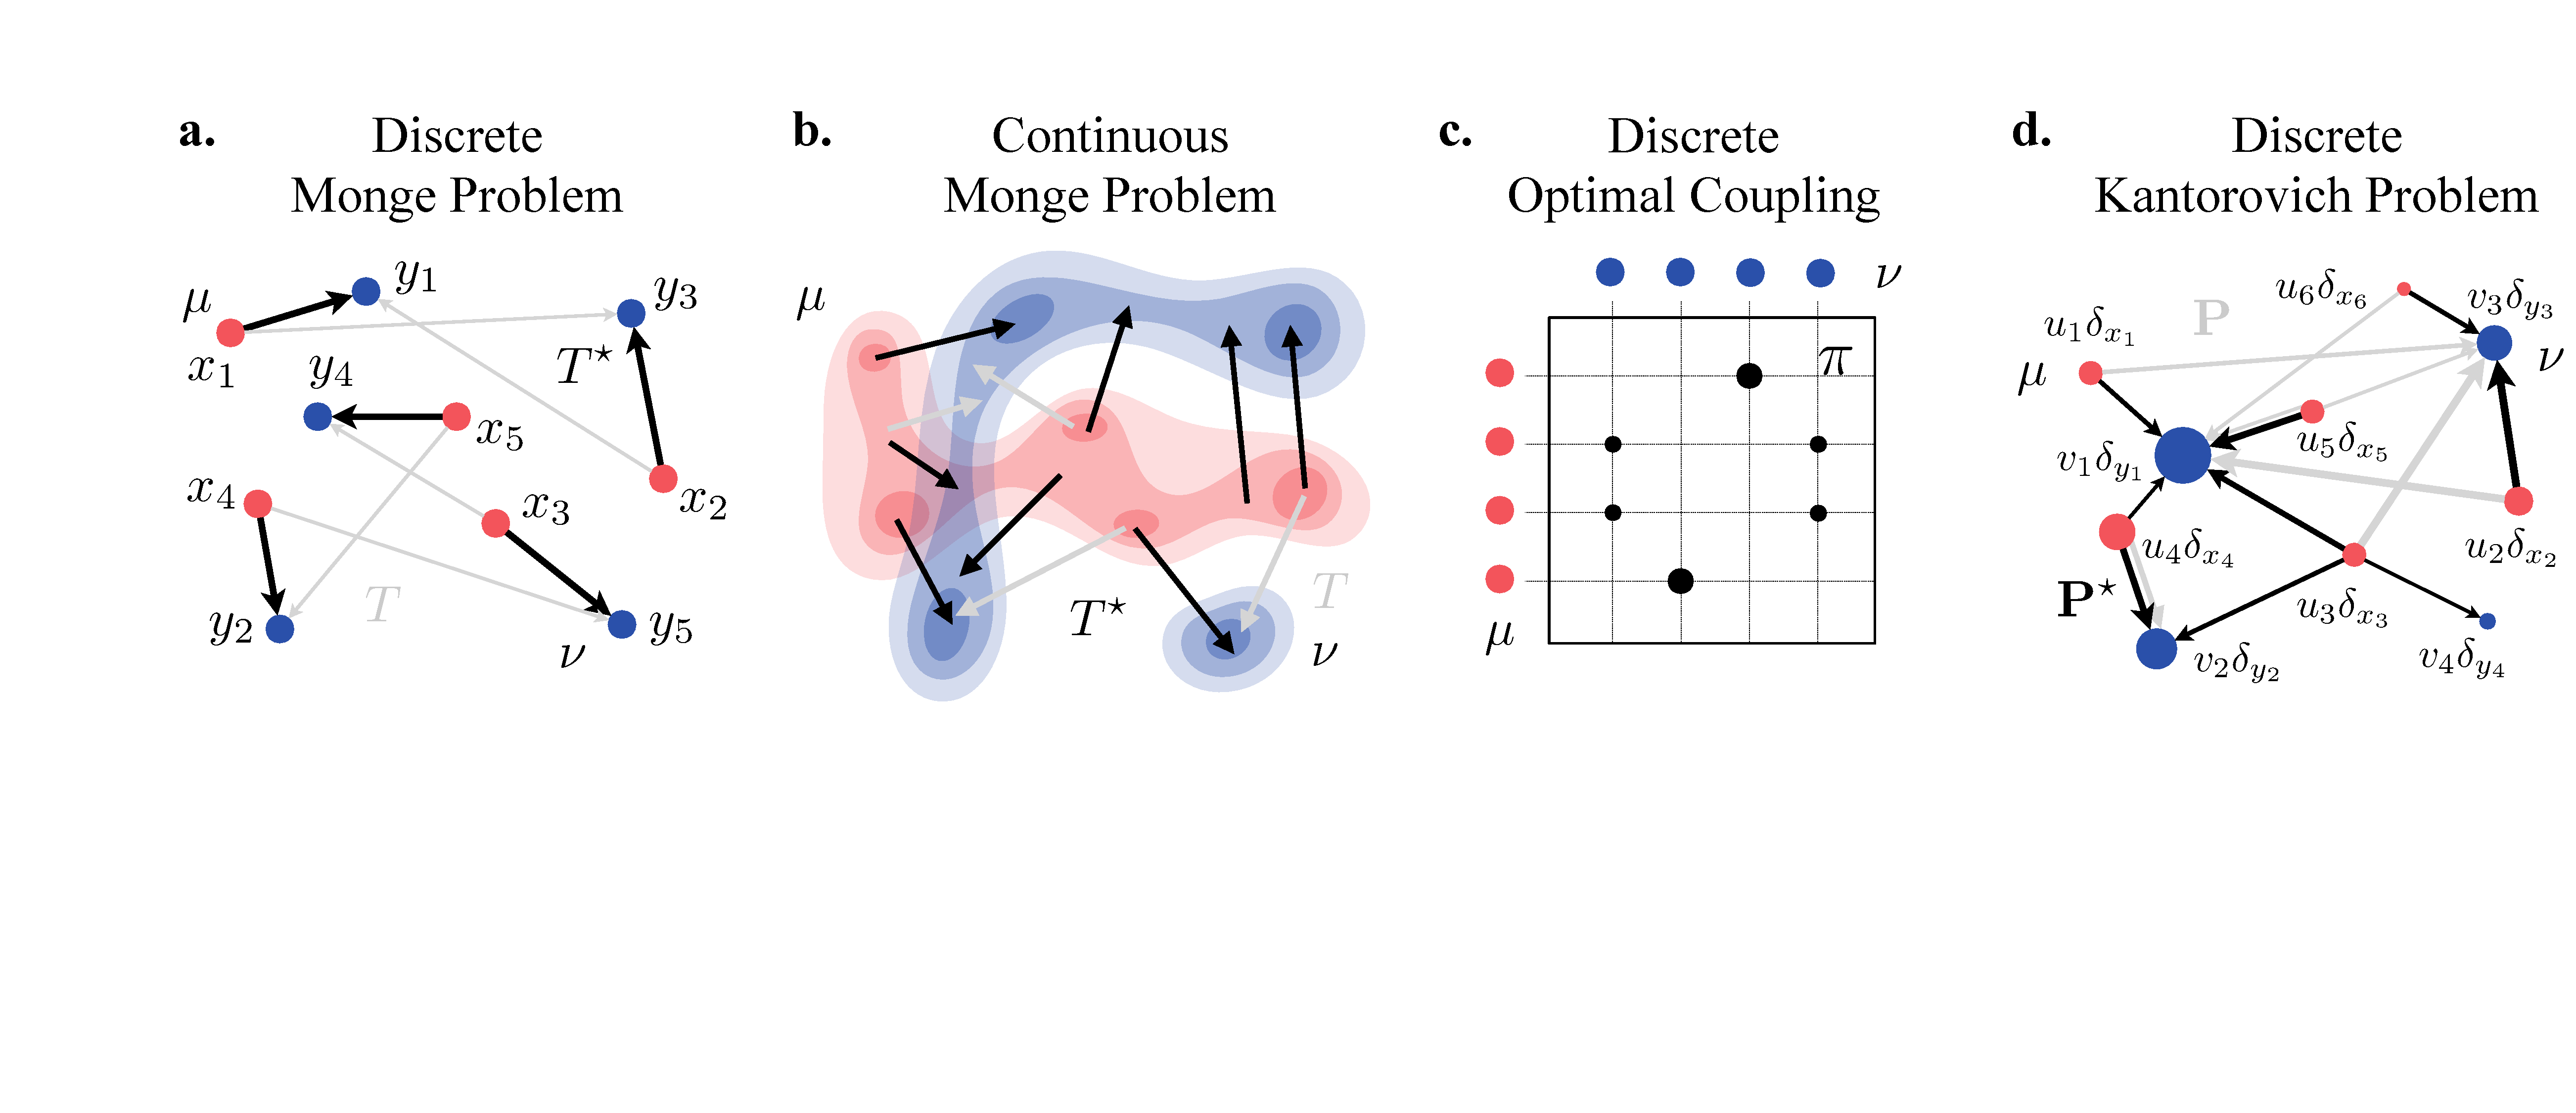
\includegraphics[width=\textwidth]{figures/fig_ot_background.pdf}
  \caption{\textbf{Overview on different formulations of the static OT problem for discrete and continuous measures.} Monge map for \textbf{a.} discrete and \textbf{b.} continuous measures $\mu, \nu$. The optimal map $T^\star$ minimizes \eqref{eq:monge}. \textbf{c.} Optimal coupling $\pi$ \eqref{eq:kantorovich} for discrete measures $\mu$ and $\nu$. \textbf{d.} Mass splitting principle of the Kantorovich relaxation for discrete measures $\mu$ and $\nu$ of the optimal transport plan $\bP^\star$ and a non-optimal plan $\bP$. Figure adapted from \citet{peyre2019computational}.}	
  \label{fig:ot_principles}
\end{figure}

\subsection{Monge Problem} \label{sec:background_monge}

In the 18th century "M{\'e}moire sur la th{\'e}orie des d{\'e}blais et des remblais", Gaspard Monge sets out to solve what is now known as the \citeauthor{monge1781histoire} problem, posing a seemingly simple, yet fundamentally complex question: Given two quantities of mass located at two different sites, what is the most efficient way to transport one into the other?
In more formal terms, provided with two measures $\mu, \nu\in \mathcal{P}(\mathbb{R}^d)$, here restricted to measures supported on $\mathbb{R}^d$, \citeauthor{monge1781histoire}'s initial approach was to find a map $T$ that pushes one mass onto the other in a way that minimizes the total cost of transport.
Given a measurable const function $c: \mathcal{X} \times \mathcal{Y} \rightarrow \mathbb{R}$, the \citeauthor{monge1781histoire} problem then reads
\begin{equation}\label{eq:monge}
T^\star := \arg\inf_{T\sharp\mu=\nu}\int_{\mathbb{R}^d} c(x, T(x)) d\mu(x)\,.
\end{equation}
For two discrete measures $\mu=\sum_{i=1}^n u_i \delta_{x_{i}}, \nu=\sum_{j=1}^m v_j \delta_{y_{j}}$, it seeks a transport map $T: \mathcal{X} \rightarrow \mathcal{Y}$ associating each source point $x_i$ to a target point $y_j$ (see \cref{fig:ot_principles}a for the discrete and \cref{fig:ot_principles}b for the continuous setting).
% TODO: Add more butter.
The existence of $T^\star$ is guaranteed under fairly general conditions \citep[Theorem 1.22]{santambrogio2015optimal}, which require that $\mu$ and $\nu$ have finite $\ell_2$ norm, and that $\mu$ puts no mass on $(d-1)$ surfaces of class $\mathcal{C}_2$, 
% TODO: Check the statement below.
i.e., the family of continuous functions that have both a continuous first and a continuous second derivative.


\subsection{Kantorovich Relaxation} \label{sec:background_kantorovich}

It was not until the 20th century, however, that the concept found a more tractable development. In \citeyear{kantorovich1942transfer}, Leonid \citeauthor{kantorovich1942transfer} provided a relaxation to this non-convex and difficult-to-solve problem.
Instead of the deterministic matching proposed by \citeauthor{monge1781histoire}, Kantorovich considered probabilistic correspondences that allow for the transportation of mass from a single source point to various target points (mass splitting), resulting in the problem formulation
% TODO: Introduce P_{\gX \sharp}.
\begin{equation} \label{eq:kantorovich}
    W(\mu, \nu) \defeq \inf_{\pi\in \Pi(\mu,\nu)}\iint c(x, y) \pi(x, y)\mathrm{d}x\mathrm{d}y,
\end{equation}
where $\Pi(\mu, \nu) \defeq \left\{\pi \in \gP(\mathcal{X} \times \mathcal{Y}): P_{\gX \sharp} \pi=\mu \, \text { and } \, P_{\gY \sharp} \pi=\nu\right\}$ is the set of couplings on $\mathbb{R}^d\times\mathbb{R}^d$ with respective marginals $\mu, \nu$. Given the optimal transport coupling $\pi$, the resulting distance $W(\mu, \nu)$ between $\mu$ and $\nu$ is known as the Wasserstein distance.
A visualization of the discrete setting is provided in \cref{fig:ot_principles}c.

For his work, \citeauthor{kantorovich1942transfer} received the Nobel Prize in economics. The connection of \acrshort{OT} to basic questions in economy becomes clear when interpreting $\mu$ as a density of resource units, and $\nu$ a density of factories, where the coupling $\pi$ denotes the optimal transportation plan of distributing resources to factories.

Despite its elegance, the Wasserstein distance \eqref{eq:kantorovich} presents a computationally challenging optimization problem. A partial remedy proposed by \citet{cuturi2013sinkhorn} is to solve regularized optimal transportation problems for an approximate solution. One example of an effective regularization is entropy regularization: For $\varepsilon\geq0$, set 
\begin{equation} \label{eq:ot-entropy}
\We(\mu,\nu) = \inf_{\pi\in \Pi(\mu,\nu)}\iint c(x, y) \pi(x, y)\mathrm{d}x\mathrm{d}y  \,-\varepsilon H(\pi),
\end{equation}
where $H(\pi) \defeq - \iint \pi(x, y)\log\pi(x, y)\mathrm{d}x\mathrm{d}y$ is the entropy of coupling $\pi$. 
Notice that the definition above reduces to the usual Wasserstein distance \eqref{eq:kantorovich} when $\varepsilon=0$.
When instantiated on finite discrete measures, such as $\mu=\sum_{i=1}^n u_i\delta_{x_i}$ and $\nu=\sum_{j=1}^m v_j\delta_{y_j}$, \eqref{eq:kantorovich} translates to a linear program
\begin{equation}\label{eq:ot-reg}
\We(\mu,\nu) \defeq \min_{\bP\in U(\mu,\nu)} \dotp{\bP}{[\|x_i - y_j\|^2]_{ij}}  \,-\varepsilon H(\bP),
\end{equation}
where $H(\bP) \defeq -\sum_{ij} \bP_{ij} (\log \bP_{ij} - 1)$ and the polytope $U(\mu,\nu)$ is the set of $n\times m$ matrices $\{\bP\in\mathbb{R}^{n \times m}_+, \bP\mathbf{1}_m = \mu, \bP^T \mathbf{1}_n=\nu\}$.
Regularization with an entropy term results in a significantly more efficient optimization \citep{cuturi2013sinkhorn} and differentiability w.r.t. the inputs.
As a consequence, \ref{eq:ot-reg} is commonly used as a loss function or evaluation metric in machine learning applications, e.g., for structured prediction \citep{frogner2015learning,janati2020multi} or generative model fitting \citep{arjovsky2017wasserstein, salimans2018improving, genevay2018learning}.
While setting $\varepsilon>0$ yields a faster and differentiable proxy to approximate $W_{0}$, it introduces a bias, since $\We(\mu,\mu)\ne 0$ in general.

\subsection{Kantorovich Duality} \label{sec:background_dual}

The Kantorovich formulation \eqref{eq:kantorovich} is a \emph{convex} problem on $\gP(\mathcal{X} \times \mathcal{Y})$ and thus admits a dual formulation introduced by \citet{kantorovich1942transfer}, i.e., a constrained concave maximization problem defined as
\begin{equation} \label{eq:kantorovich-dual}
    W(\mu, \nu)\defeq\sup _{(f, g) \in \Phi_{c}} \int f \mathrm{~d} \mu+\int g \mathrm{~d} v,
\end{equation}
\looseness -1 where the set of admissible dual potentials is given by $\Phi_c \defeq \{(f, g) \in L^{1}(\mu) \times L^{1}(\nu): f(x)+g(y) \leq c(x,y)$, $\forall(x, y)\, d\mu \otimes d\nu \text{ a.e.}\}$.
$(f, g)$ is thus a pair of continuous functions, often referred to as \emph{Kantorovich potentials}.
An informal interpretation of \eqref{eq:kantorovich-dual} was provided by \citet{caffarelli2003monge}, revisiting the connection of \acrshort{OT} to economics: 
A logistics company is concerned with transporting products from each resource unit $x$ to a factory $y$. The transportation company charges $f(x)$ for loading resources at point $x$ and $g(y)$ for unloading it at destination $y$ but is constrained to charge $f(x)+g(y) \le c(x,y)$. In order to arrange prizes $f$ and $g$ that increase profit, they thus maximize objective \eqref{eq:kantorovich-dual}.

The Kantorovich duality \eqref{eq:kantorovich-dual} is a core pillar of \acrlong{OT}, powerful due to its generality and computationally attractive as it is easier to store two functions $(f, g)$ than an entire coupling $\pi$.
In the following, we will introduce the concept of $c$-transforms, a useful machinery to reduce \eqref{eq:kantorovich-dual} even further into an optimization problem over only one instead of two dual potentials.
\begin{definition}[$c$-transform] \label{eq:c-transform} 
	$c$-transforms (also called $c$-conjugate functions) are generalizations of the Legendre transform from convex analysis defined as
\begin{align*} \tag{c-transform}
	& \forall y \in \gY, \quad f^c(y) \defeq \inf _{x \in \gX} c(x, y)-f(x) \,. \\
	\intertext{The definition of $f^c$ is also often referred to as a "Hopf-Lax formula". Similarly to the $c$-transform of $f : \gX \rightarrow \mathbb{R}$, we can define the $\bar{c}$-transform of $g : \gY \rightarrow \bar{\mathbb{R}}$ by}
	& \forall x \in \gX, \quad g^{\bar{c}}(y) \defeq \inf _{y \in \gY} c(x, y)-g(y) \,,
\end{align*}
where $\bar{c}(y, x) = c(x, y)$. 
\end{definition}
Further, $f$ is a \textit{$\bar{c}$-concave} function if there exists a $g$ such that $f = g^{\bar{c}}$, and analogously, a function $g$ is said to be \textit{$c$-concave} if there is a function $f$ such that $g = f^c$.
When $\gX = \gY$ and $c$ is symmetric no distinction between $c$ and $\bar{c}$ is necessary.

Using the concept of $c$-transforms, we can reduce \eqref{eq:kantorovich-dual} to a single potential: Assume we keep dual potential $f$ fixed and given the constraint of the dual formulation\eqref{eq:kantorovich-dual}
\begin{align*}
  f(x)+g(y) & \leq c(x, y) \\
  g(y) & \leq c(x, y)-f(x)\,, \\
  \intertext{we can see that the "best" potential $g$ is given by the \cref{eq:c-transform} of $f$ }
  \label{eq:best_g} g(y) & \leq \inf _x c(x, y)-f(x).
\end{align*} 
Then, doing an alternate optimization on either $f$ or $g$, we replace the dual potentials $(f, g)$ with $(f, f^c)$, and then $(f^{c\bar{c}}, f^c)$, whilst preserving the constraints and increasing the value of the integrals of \eqref{eq:kantorovich-dual}.  
Although one could continue this alternate optimization further, the invariance property $f^{c\bar{c}c} = f^c$ for any $f$ shows that one can only "improve" once the dual potential using $c$-transforms, resulting in the semi-dual formulation of \acrlong{OT}
\begin{equation} \label{eq:semi-dual}
  f^\star \defeq \arg\max_{f\, c\text{-concave}} \int f \textrm{d}\mu + \int f^c\textrm{d}\nu\,,
\end{equation}
where $f^\star$ is the optimal dual function and $c$-concave.
% While \eqref{eq:kantorovich-dual} was historically derived based on the duality  principle by \citet{kantorovich1942transfer}, an alternate derivation involves the study of such $c$-concave functions. 
% Following \citet[Theorem 1.39]{santambrogio2015optimal}, ... c-superdifferential ...
% \begin{equation*}
%	\supp(\pi) \subset \left\{(x, y) \in \gX \times \gY: f(x)+f^c(y)=c(x, y)\right\}\,
% \end{equation*}
% and
% \begin{equation*}
%	\int_\gX f \mathrm{d} \mu+\int_\gY f^c \mathrm{~d} \nu=\int_{\gX \times \gY}\left(f(x)+f^c(y)\right) \mathrm{d} \pi(x, y)=\int_{\gX \times \gY} c(x, y) \mathrm{d} \pi(x, y)\.
% \end{equation*}
% Thus, the solutions of \eqref{eq:kantorovich} and \eqref{eq:kantorovich-dual} are equivalent.
\subsection{Geometry of Optimal Transport}
\label{sec:background_brenier}

Following \citet{gangbo1996geometry}, $f^\star$ can be linked to the optimal transport map $T^\star$ via the following result:
\begin{theorem}[Gangbo-McCann Theorem] \label{thm:gangbo-mccann}
	Given a cost function $c$, the relationship between the optimal transport map $T^\star : \gX \rightarrow \gX$ and the $c$-concave function $f^\star$ denoting the optimal dual potential is given by the expression 
	\begin{equation}
		T^{\star}(x)=\nabla_1 c(x, \cdot)^{-1} \circ \nabla f^{\star}(x)\,.
	\end{equation}
	Thus, map $T$ depends explicitly on the gradient of the cost, or rather on its inverse map \citep{gangbo1995optimal}. 
	
	Following \citet{gangbo1996geometry} and considering translation-invariant costs\footnote{A cost is translation-invariant if $c(x,y) = h(x-y)$ for $h(z) = h(-z)$.} generated by a convex potential $h: \mathbb{R}^d \rightarrow \mathbb{R}$, i.e., c(x, y)=h(x-y), this reduces to
	\begin{equation} \label{eq:gangbo_h}
		T^{\star}(x)=x-\nabla h^* \circ \nabla f^{\star}(x)\,,
	\end{equation}
	where $h^*$ is the Legendre-transform of $h$ given by
	\begin{equation} \label{eq:legendre}
		\tag{Legendre transform}
		\forall z, \quad h^*(z) \defeq \sup _x \langle x, z\rangle-h(x)\,.
	\end{equation}

\end{theorem}
\begin{proof}
\citet[Theorem 1.39]{santambrogio2015optimal} proves that the solutions of \eqref{eq:kantorovich} and \eqref{eq:kantorovich-dual} are equivalent, i.e.,
\begin{equation*}
	\int_\gX f \mathrm{d} \mu+\int_\gY f^c \mathrm{~d} \nu=\int_{\gX \times \gY}\left(f(x)+f^c(y)\right) \mathrm{d} \pi(x, y)=\int_{\gX \times \gY} c(x, y) \mathrm{d} \pi(x, y)\,.
\end{equation*}
Then, a point $(x_0, y_0)$ in the coupling $\pi$, i.e., $(x_0, y_0) \in \supp(\pi)$, necessarily satisfies the constraint of the dual problem \eqref{eq:kantorovich-dual}
\begin{align*}
\pi^{\star}\left(x_0, y_0\right)>0 & \Leftrightarrow f^{\star}\left(x_0\right)+g^{\star}\left(y_0\right)=c\left(x_0, y_0\right). \\
\intertext{Replacing $g$ by the $c$-transform of $f$, we have}
& \Leftrightarrow f^{\star}\left(x_0\right)+ f^{c\star}\left(y_0\right)=c\left(x_0, y_0\right) \\
& \Leftrightarrow f^{c\star}\left(y_0\right)=c\left(x_0, y_0\right)-f^{\star}\left(x_0\right). \\
\intertext{Yet, by definition of the $c$-transform, $f^{c\star}$ is given by}
& \Leftrightarrow f^{c\star}\left(y_0\right)= \inf_z c\left(z, y_0\right)-f^{\star}\left(z\right).
\end{align*}
Thus, $x_0$ is a minimizer of the above expression and $\nabla_1 c\left(x_0, y_0\right)=\nabla f^{\star}\left(x_0\right)$.  
Therefore, after inversion, we have $y_0=\nabla_1 c(x, \cdot)^{-1} \circ \nabla f^{\star}(x)$ and
\begin{equation*}
		T^{\star}(x)=x-\nabla h^* \circ \nabla f^{\star}(x)\,.
	\end{equation*}
Applying this result to $c(x, y) = h(x-y)$, we get 
\begin{align*}
  \nabla_1 c(x, y) & =\nabla h(x-y) \\
  \nabla_1 c(x, \cdot) & =\nabla h(x-\cdot) \\
  \nabla_1 c(x, \cdot)^{-1} & =x-(\nabla h)^{-1}(\cdot)\,. \\ 
\intertext{Note that $(\nabla h)^{-1}$ is equivalent to $\nabla h^*$ with the convex conjugate $h^*$ and thus,}
  \nabla_1 c(x, \cdot)^{-1} & =x-\nabla h^*(\cdot)\,.	
\end{align*}
\end{proof}
Alternative formulations that relate the Kantorovich setting (with general costs) \eqref{eq:kantorovich-dual} to that of Monge \eqref{eq:monge} were proposed by \citet{ruschendorf1991bounds, ruschendorf1991frechet, caffarelli2017allocation}. \\

% Problem \eqref{eq:kantorovich-dual} allows us to characterize optimal transport plans that emerge as the solution to the Kantorovich optimal transportation problem \eqref{eq:kantorovich} and show sufficient conditions for the existence of optimal transport maps.
The case of the squared Euclidean cost\footnote{For elegance, we consider $c(x, y) = \frac{1}{2}\norm{x-y}^2$ instead of $c(x, y) = \norm{x-y}^2$.} $c(x, y) = \frac{1}{2}\norm{x-y}^2$ in $\gX = \gY = \mathbb{R}^d$ deserves a special attention. 
Taking advantage of the particular form of the quadratic cost function, we can expand the constraint of \eqref{eq:kantorovich-dual} such that 
\begin{equation*}
	f(x)+g(y) \leq \frac{1}{2}\|x-y\|_2^2 \Longleftrightarrow  {\left[\frac{1}{2}\|x\|_2^2-f(x)\right]+\left[\frac{1}{2}\|y\|_2^2-g(y)\right] \geq\langle x, y\rangle}
\end{equation*}
and subsequently reparameterize $\varphi(x) \defeq \frac{1}{2}\|x\|_2^2-f(x)$ and $\psi(y) \defeq \frac{1}{2}\|y\|_2^2-g(y)$.
Mirroring the same logic as for the $c$-transform, we derive the semi-dual in the Euclidean setting 
\begin{equation} \label{eq:dual-cvx}
  \inf_{\varphi\, \text{convex}} \int \varphi \textrm{d}\mu + \int \varphi^*\textrm{d}\nu\,.
\end{equation}
Following the double convexification trick as outlined in \citet[Lemma 2.10]{villani2021topics}, we see that applying the \ref{eq:legendre} twice yields function pair $(\varphi^{**},\varphi^{*})$. As each of them is defined as the supremum of a family of linear functions, the result is an optimization problem over two convex \acrlong{lsc} functions.

Similarly, for the special case of the squared Euclidean distance the \cref{thm:gangbo-mccann} \eqref{eq:gangbo_h} with $h=\frac{1}{2}\|\cdot\|_2^2 $ implies that $\nabla h=\nabla h^*=\mathrm{Id}$, and thus
\begin{equation*}
	T(x)=x-\nabla f(x)=\nabla\left(\frac{1}{2}\|x\|^2_2-f(x)\right)(x)=\nabla \varphi(x),
\end{equation*}
where we again reparameterize $\varphi(x) \defeq \frac{1}{2}\|x\|^2_2-f(x)$ and $\varphi(x) = \frac{1}{2}\|x\|_2^2-f(x)$ can be shown to be convex.

This connection presents a well known fact that has been investigated first by \citeauthor{brenier1987decomposition}, establishing for the special case of the Euclidean distance the equivalence of the Monge \eqref{eq:monge} and Kantorovich formulation  \eqref{eq:kantorovich}, the uniqueness of the optimal coupling $\pi$, and instantiating that there must exist a unique (up to the addition of a constant) potential $\varphi^\star:\mathbb{R}^d\rightarrow \mathbb{R}$ such that $T^\star = \nabla \varphi^\star$. 
This theorem has far-reaching implications: When seeking optimal transport maps, it is sufficient, to restrict the computational effort to seek a "good" convex potential $\varphi$, such that its gradient pushes $\mu$ towards $\nu$. 
Let us state the celebrated \citeauthor{brenier1987decomposition} theorem \citeyearpar{brenier1987decomposition} in more formal terms:
\begin{theorem}[Brenier Theorem] \label{thm:brenier}
	In the setting where both $\mathcal{X}$ and $\mathcal{Y}$ are equal to $\mathbb{R}^d$, and the cost function $c(x, y) = \norm{x-y}^2$ is employed, and at least one of the two input measures $\mu$ possesses a density $p_\mu$ in relation to the Lebesgue measure, then there exists a unique optimal solution $\pi$ in the Kantorovich formulation \eqref{eq:kantorovich}.
	This solution is exclusively supported on the graph $(x, T(x))$ of Monge map $T: \mathbb{R}^d \rightarrow \mathbb{R}^d$.
	In other terms, we can express $\pi$ as $(\operatorname{Id}, T)_{\sharp} \alpha$, meaning that for any function $h$ belonging to the set $\forall h \in \mathcal{C}(\mathcal{X} \times \mathcal{Y})$, the following equality holds
	$$
	\quad \int_{\mathcal{X} \times \mathcal{Y}} h(x, y) \mathrm{d} \pi(x, y)=\int_{\mathcal{X}} h(x, T(x)) \mathrm{d} \mu(x).
	$$
Moreover, this map $T$ is uniquely determined by the gradient of a convex function $\varphi$, denoted as $T(x)=\nabla \varphi(x)$. The function $\varphi$ is the unique convex function, up to an additional constant, for which $(\nabla \varphi)_{\sharp} \mu=\nu$.
\end{theorem}
\begin{corollary}
	Under the assumption of \cref{thm:brenier}, $\nabla \varphi$ is the unique solution to the Monge transportation problem \eqref{eq:monge}, i.e.,
	\begin{equation}
		\int_{\mathbb{R}^d} \norm{x-\nabla \varphi(x)}^2 \mathrm{d}\mu(x) = \inf_{T_\sharp \mu = \nu} \int_{\mathbb{R}^d}\norm{x - T(x)}^2 \mathrm{d}\mu(x).
	\end{equation}
\end{corollary}
%To avoid confusion, we again note that the relationship between this convex function $\varphi$ and the dual potential $f$ that solves \eqref{eq:kantorovich-dual} is given $\varphi(x)$ as $\frac{\|x\|^2}{2}-f(x)$.

\cref{thm:brenier} by \citet{brenier1987decomposition, brenier1991polar} has been exploited to propose neural OT solvers ~\citep{taghvaei20192, makkuva2020optimal, korotin2021wasserstein, bunne2022proximal, alvarez2021optimizing, mokrov2021large, amos2023amortizing} and recurrently permeates this thesis (see  \cref{cha:cellot} and \ref{cha:condot}), proving its essential nature in multiple instances and modern developments of optimal transport.
Further, it presents an elegant way to solve the Monge problem in a geometric sense and has profound implications for the dynamic version of the problem, which we will study next.


\section{Dynamic Optimal Transport} \label{sec:background_ot_dynamic}

\begin{figure}[t]
  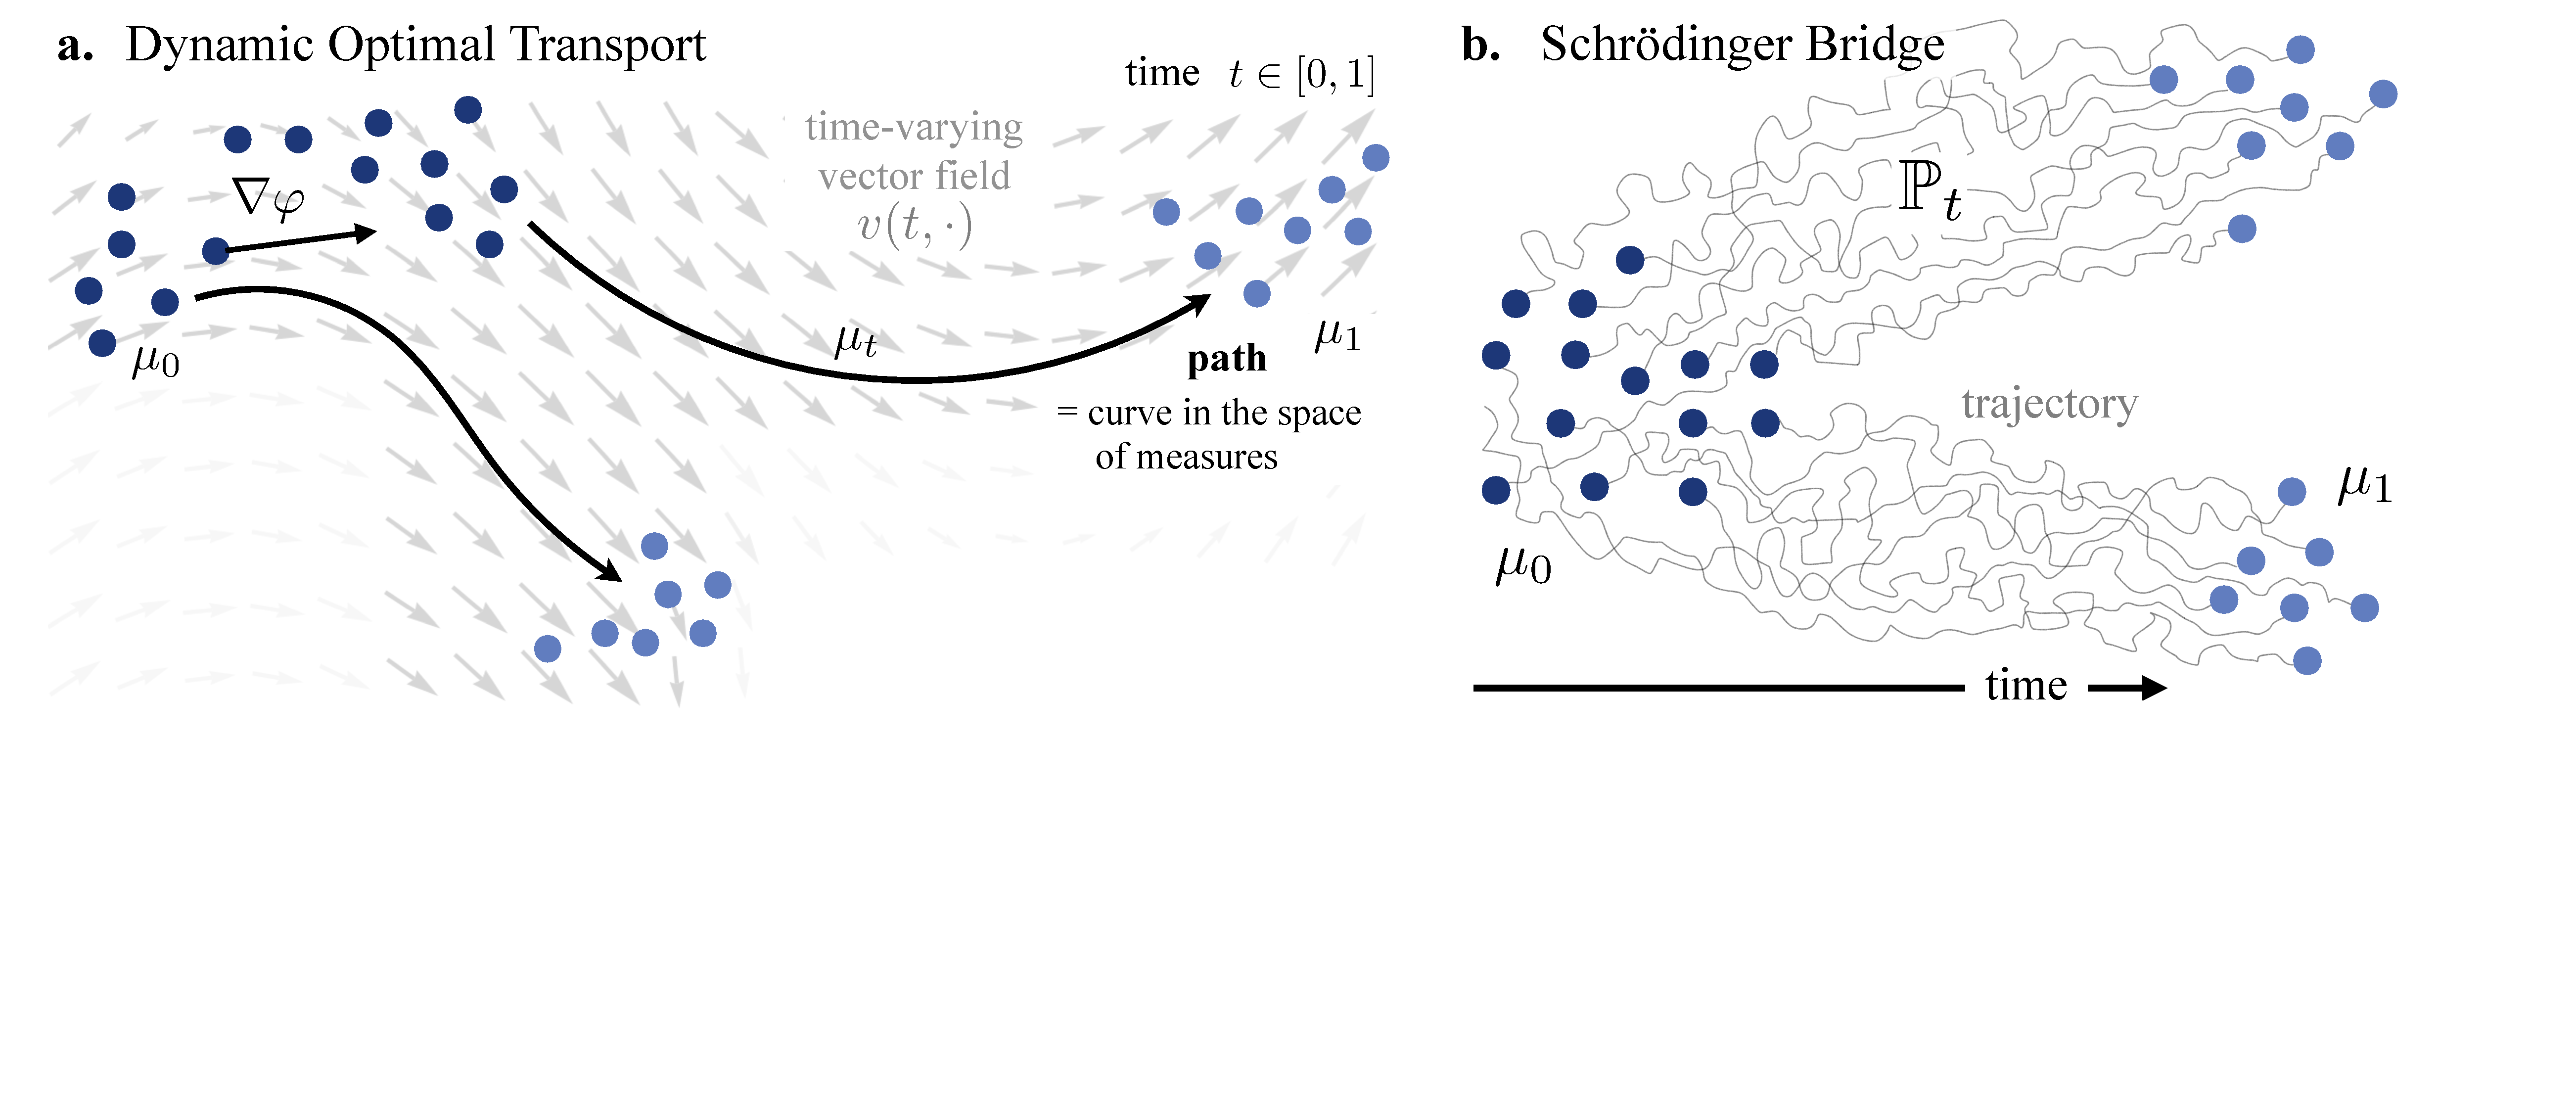
\includegraphics[width=\textwidth]{figures/fig_dynamic_ot_background.pdf}
  \caption{\looseness -1 \textbf{Overview on different formulations of the dynamic OT problem.} \textbf{a.} We can model the evolution of a measure $\mu_t$ over time as minimal path on a time-varying vector field $v(t, \cdot)$ or according to the gradient of a convex potential $\nabla \varphi$. \textbf{b.} Alternatively, taking a stochastic perspective, we can study the dynamic formulation of the entropy-regularized \acrshort{OT} problem \eqref{eq:ot-entropy} and find a stochastic process $\mathbb{P}_t$ that describes the particle dynamics from $\mu_0$ to $\mu_1$.}	
  \label{fig:dynamic_ot_background}
\end{figure}

We have hitherto engaged with the \emph{static} \acrlong{OT} problem, establishing a solid foundation upon which to build more desirable dynamic formulations. In fact, the roots of these dynamic formulations are embedded within the static \acrshort{OT} framework: As posited by \citet{benamou2000computational}, the dynamic formulation "was already implicitly contained in the original problem addressed by \citeauthor{monge1781histoire}", where "eliminating the time variable was just a clever way of reducing the dimension of the problem." When reintroducing time in the dynamic version, the optimal transport map becomes a time-dependent flow capable of describing the evolution of a measure over time.

In this section, we will cover several perspectives and frameworks of the \textbf{dynamic} \acrshort{OT} problem: As mentioned earlier, the \citeauthor{brenier1987decomposition} theorem  forms a critical bridge that connects the static and dynamic formulation, perpetuated in the Monge-Amp{\`e}re equation.
Further, \citet*{benamou2000computational} introduce how the dynamic point of view offers an alternate and intuitive interpretation of optimal transport with links to fluid dynamics. The resulting framework surprisingly leads to a convex optimization problem that can be parameterized through continuous normalizing flows \citep{tong2020trajectorynet, chen2018neural} or flow matching frameworks \citep{lipman2023flow, liu2022flow, pooladian2023multisample, albergo2023stochastic}.
We further highlight the connections of \acrshort{OT} to \acrshortpl{PDE} such as Fokker-Planck-like equations through the \citeauthor*{jordan1998variational} scheme.
Lastly, moving beyond PDEs and taking a stochastic control perspective, we will introduce the notion of the Schr\"odinger bridge problem.


\subsection{Monge-Amp{\`e}re Equation} \label{sec:background_monge_ampere}

% Caffarelli's regularity theorems from the 1990s represented a major breakthrough in our understanding of the Monge-Amp{\`e}re equation, a highly nonlinear, quintessential partial differential equation, that for instance is used to construct surfaces of prescribed Gaussian curvature. Important existence results were established by Alexandrov, and earlier central properties had been shown by Caffarelli in collaboration with Nirenberg and Spruck, with further key contributions by Evans and Krylov. Caffarelli however closed the gap in our understanding of singularities by proving that the explicitly known examples of singular solutions are the only ones.

% Caffarelli has, together with collaborators, applied these results to the Monge-Kantorovich optimal mass transportation problem, based on previous work by Brenier. Caffarelli and Vasseur gave deep regularity results for the quasi-geostrophic equation in part by applying the exceptionally influential paper by Caffarelli and Silvestre on the fractional Laplacian.
As a direct consequence of \cref{thm:brenier}, if $T(x) = \nabla \varphi(x)$, $\varphi$ being smooth and strictly convex, and $\mu$ and $\nu$ absolutely continuous with densities $p_\mu$ and $p_\nu$, we can express $T_\sharp \mu = \nu$ in a nonlinear \acrfull{PDE} form. More concretely, as a consequence of a simple change-of-variable computation, $\varphi$ is a solution of the Monge-Amp{\`e}re equation that reads
\begin{equation} \label{eq:monge_ampere}
	\operatorname{det}\left(\partial^2 \varphi(x)\right) p_\nu(\nabla \varphi(x))=p_\mu(x),
\end{equation}
where $\partial^2 \varphi(x) \in \mathbb{R}^{d \times d}$ is the Hessian of $\varphi$, describing the continuous evolution from $\mu$ to $\nu$.
First studied by \citeauthor{monge1781histoire} in \citeyear{monge1781histoire} and later by \citeauthor{ampere1819memoire} in \citeyear{ampere1819memoire}, this nonlinear partial differential equation arises in several problems from analysis to geometry, for example, in the Weyl and Minkowski problems in differential geometry of surfaces. 
The regularity of the solutions of \eqref{eq:monge_ampere}, with implications on regularity results of the optimal transport map $T$, has been subject of a series of works by \citeauthor{caffarelli1990interior} in the \citeyear{caffarelli1990interior}s, for which he was awarded the Abel Prize in 2023, as well as more recently by \citeauthor{figalli2017monge}, recognized with the Fields Medal in 2018.


\subsection{Benamou-Brenier Formulation} \label{sec:background_benamou_brenier}

Avoiding solving \eqref{eq:monge_ampere} directly, \citet{benamou2000computational} introduce an alternative numerical framework by connecting the optimal mass transfer problem to continuum mechanic frameworks.
Deviating from the previous notation of $(\mu, \nu)$, in the following sections we study the dynamic problem via the evolution from measure $\mu_0$ at time $t=0$ to $\mu_1$ at $t=1$. 
In the setting $\gX = \gY = \mathbb{R}^d$ with the squared Euclidean cost $c(x, y) = \norm{x-y}^2$, the solution of \eqref{eq:kantorovich} then coincides with finding the minimal path $(\mu_t)_{t=0}^1$, or more concretely, a curve in the space of measures, minimizing a total length.  
Such path $\mu_t$ can be described through a time-varying vector field $v(t, \cdot)$ which moves particles around, satisfying the continuity equation in fluid dynamics or conservation of mass formula
\begin{equation} \label{eq:continuity_equation}
	\frac{\partial \mu_t}{\partial t}+\nabla\left(\mu_t v\right)= 0, \qquad \mu_{t=0}=\mu_0, \mu_{t=1}=\mu_1\,,
\end{equation}
where the vector field $v(t, \cdot)$ denotes the speed and $\mu_t v(t, \cdot) = J_t$ corresponds to the momentum.
Reformulating the optimal transportation problem in a differential way, an "Eulerian" formulation inspired by fluid mechanics, will be crucial for the subsequent study of dynamical problems.
Every curve $\mu_t$ describing the evolution of the measure over time can be interpreted as the fluid flow along a family of vector fields. We are searching for the vector field $v(t, \cdot)$ that (i.) satisfies the conservation of mass \eqref{eq:continuity_equation}, and (ii.) minimized the path length.
The infinitesimal length of such a vector field can be computed via 
\begin{equation} \label{eq:vector_field_length}
	\left\|v\right\|_{\ell^2\left(\mu_t\right)}=\left(\int_{\mathbb{R}^d}\left\|v(t, x)\right\|^2 \mathrm{~d} \mu_t(x)\right)^{1 / 2}.
\end{equation}
resulting, in the case of $\gX = \gY = \mathbb{R}^d$ and $c(x, y)=\|x-y\|^2$, in the minimal-path reformulation of \eqref{eq:kantorovich}
\begin{align}  \label{eq:benamou_brenier}
	W\left(\mu_0, \mu_1\right)=& \inf _{(\mu_t, v)} \int_0^1 \int_{\mathbb{R}^n}\frac{1}{2}\norm{v(t, x)}^2 d\mu_t(x) d t \\
	& \nonumber \frac{\partial \mu_t}{\partial t}+\nabla \cdot(v \mu_t)=0 \\
	& \nonumber \mu_{t=0}=\mu_0, \mu_{t=1}=\mu_1\, .
\end{align}
Thus, path $\mu_t$ describes the time-evolving density of a set of particles moving continuously with velocity $v(t, \cdot)$.
Taking the perspective of fluid dynamics, \eqref{eq:vector_field_length} can also be interpreted as the \emph{kinetic energy} of the particles.
The Benamou-Brenier formulation \eqref{eq:benamou_brenier} then selects the vector field $v$ that minimizes the total efforts or the total kinetic energy one has to spend in order to move particles around according to the vector field $v$. \\


A particularly important case occurs when there exists an optimal Monge map $T: \mathbb{R}^d \rightarrow \mathbb{R}^d$ with $T_\sharp \mu_0 = \mu_1$ (see \cref{thm:brenier}): The solution of the time-dependent OT problem \eqref{eq:benamou_brenier} then coincides with \citeauthor{mccann1997convexity}'s displacement interpolation between two measures.
Reciting \cref{thm:brenier}, with $T = \nabla \varphi$, $\mu_t$ is equal to \citeauthor{mccann1997convexity}'s interpolation between $\mu_0$ and $\mu_1$ given by
\begin{equation} \label{eq:mccann_interpolation}
	\mu_t = [(1-t) I+t \nabla \varphi]_\sharp \mu_0 = [(1-t) I+t T]_\sharp \mu_0\,.
\end{equation}
Despite their simplicity, this concept possesses remarkable applications beyond the realm of optimal transport \citep{bonneel2011displacement}. In particular, its interpretation as a geodesic formula in Riemannian geometry is thoroughly discussed in \citet{gangbo1996geometry} and serves as a pivotal link to the subsequent discussion.


\subsection{Jordan-Kinderlehrer-Otto Flows} \label{sec:background_jko}

The time-dependent Benamou-Brenier formulation \eqref{eq:benamou_brenier} not only provides us with a more complete description of optimal transport but also the discovery that the resulting path $(\mu_t)_{t=0}^1$ may be seen as a constant-speed geodesic interpolating between population $\mu_0$ and $\mu_1$ in the space of measures, i.e., a Wasserstein geodesic.
When studying dynamic processes in biomedicine, however, phenomena such as cellular differentiation in developmental processes, tissue formation, or cell migration involve intricate spatiotemporal dynamics that cannot be adequately captured by solely studying the interpolation between two measures $\mu_0$ and $\mu_1$.
Instead, many phenomena in biology and physics can be modeled through an energy functional $J$ such that the minimization of $J$ describes the observed dynamics of the studied system ---a concept known as gradient flows.
At their core, gradient flows provide a powerful framework for understanding the evolution of functions or systems towards an optimal state through the direction of the steepest descent of a function $J$. 
More concretely, gradient flows capture the intuitive idea of objects moving in a direction that decreases their energy, seeking a state of minimum potential or maximum stability. 
In the following, we will study gradient flows in the Euclidean setting before considering generalizations to arbitrary measures that allow studying the evolution of populations over time.

% It is natural to derive various partial differential equations (PDEs) as gradient flows of certain energy functionals.

\paragraph{Euclidean case.}
Considering the evolution of a vector $x$ over time in Euclidean space. Provided with a smooth functional $J$, this can be realized through the standard gradient descent (forward) scheme
\begin{equation*}
	x_{t+1} \defeq x_{t}-\tau \nabla J\left(x_{t}\right),
\end{equation*}
where $\tau$ is the step size. The resulting sequence ${x_0, \dots, x_{t-1}, x_{t}, x_{t+1}, \dots, x_T}$ then describes the trajectory of a single particle $x$ over time.
For non-smooth functions, on can resort to a proximal scheme, i.e.,
\begin{equation*}
	x_{t+1} \defeq \operatorname{Prox}_{\tau J}^{\|\cdot\|}\left(x_{t}\right) \defeq \arg\!\min_x \frac{1}{2\tau}\left\| x-x_t\right\|^2+ J(x).
\end{equation*}
The proximal scheme can thus be seen as a \emph{backward} Euler discretization of the gradient flow.

\paragraph{Wasserstein case.}
When studying the evolution of a population or measure $\mu_t$ over time, however, we need to resort to optimal transport metrics $W(\cdot, \cdot)$ \eqref{eq:kantorovich} instead of the $\ell_2$-norm $\norm{\cdot}^2$.
Considering functionals $J$ that take a measure or population as input, a gradient flow of $\mu$ w.r.t. to $J$ can be similarly expressed through forward and backward schemes. Assuming $J(\mu) 
\defeq \int E(x) d \mu(x)$, i.e., ignoring particle interaction, the forward scheme reads
\begin{equation*}
	\mu_{t+1}\defeq\left(I-\tau \nabla E\right)_{\sharp} \mu_t
\end{equation*}
with the corresponding backward formulation defined as
\begin{equation}
	\label{eq:jko}
	\mu_{t+1}\defeq\underset{\mu}{\operatorname{argmin}} \enspace \frac{1}{2\tau}W\left(\mu, \mu_t\right)+ J(\mu).
\end{equation}
This implicit time stepping is a useful tool to construct continuous flows: In the limit $\tau \rightarrow 0$ the resulting sequence $\{\mu_t\}_{t=0}^T$ approximates a continuous flow $\mu_t$, i.e., a path in the Wasserstein space, and can thus be seen as the analogy of the usual proximal descent scheme, tailored for probability measures~\citep[p.285]{santambrogio2015optimal}

Interest in Wasserstein gradient flows was sparked by the seminal work of Jordan, Kinderlehrer, and Otto (\citeyear{jordan1998variational}) who studied diffusion processes under the lens of the OT metric \citep[see also][]{ambrosio2006gradient}. 
For a broad class of potentials, $J$ and provided with an initial distribution $\mu_0$, the resulting time-discrete, iterative variational scheme induced by the so-called \emph{JKO step} \eqref{eq:jko} reconstructs the evolution of measure $\mu_t$ over time. As $\tau \rightarrow 0$, the solution of the time-discretized gradient flow converges to the solution of a corresponding PDE, and the resulting evolutions are often referred to as \emph{JKO flows}.

\begin{table*}[t]
	\caption{Equivalence between gradient flows and PDEs where the gradient flow of flow functional $J(\mu_t)$ in Wasserstein space satisfies the corresponding PDE \citep{alvarez2021optimizing, villani2021topics}. The function $f: \mathbb{R} \rightarrow \mathbb{R}$ is convex and superlinear and $V, W: \gX \rightarrow \mathbb{R}$ are convex and sufficiently smooth.}
	\label{tab:examples_gradient_flows}
	\centering
	\adjustbox{max width=\linewidth}{%
	\begin{tabular}{lll}
	\toprule
	\textbf{Class} & \textbf{PDE} $\frac{\partial \mu_t}{\partial t} =$ & \textbf{Flow Functional} $J(\mu_t)=$ \\
	\midrule Heat Equation & $\Delta \mu_t$ & $\int \mu_t(x) \log \mu_t(x) \mathrm{d} x$ \\
	Advection & $\nabla \cdot(\mu_t \nabla V)$ & $\int V(x) \mu_t(x) \mathrm{d} x$ \\
	Fokker-Planck & $\Delta \mu_t+\nabla \cdot(\mu_t \nabla V)$ & $\int \mu_t(x) \log \mu_t(x) \mathrm{d} x+\int V(x) \mu_t(x) \mathrm{d}x $ \\
	Porous Media & $\Delta\left(\mu_t^m\right)+\nabla \cdot(\mu_t \nabla V)$ & $\frac{1}{m-1} \int \mu_t(x)^m \mathrm{~d} x+\int V(x) \mu_t(x) \mathrm{d} x$ \\
	\makecell[l]{Advection, Diffusion, \\ and Interaction} & $\nabla \cdot\left[\mu_t\left(\nabla f^{\prime}(\mu_t)+\nabla V+(\nabla W) * \mu_t\right)\right]$ & \makecell[l]{$\int V(x) \mu_t(x) \mathrm{d} x+\int f(\mu_t(x)) \mathrm{d} x$ \\ $+\frac{1}{2} \iint W\left(x-x^{\prime}\right) \mu_t(x) \mu_t\left(x^{\prime}\right)\mathrm{d} x \mathrm{d} x^\prime$} \\
	\bottomrule
	\end{tabular}
	}
\end{table*}

In fact, following \citet{otto2001geometry} on the calculus of optimal transport (\citeauthor{otto2001geometry} calculus), a large class of \acrlong{PDE} may then be viewed as gradient flows on the Wasserstein space \citep{jordan1998variational}.
For instance, the standard heat equation of physics, i.e.,
\begin{equation*}
	\frac{\partial \mu_t}{\partial t} = \Delta \mu_t,
\end{equation*}
with $\Delta$ being the spatial Laplacian, can be expressed as a gradient flow of the energy $J(\mu) = \int \mu_t(x) \log \mu_t(x) \mathrm{d} x$, i.e., Gibbs-Boltzmann's famous functional with the physical interpretation of the negative of an entropy.
Among further examples displayed in \cref{tab:examples_gradient_flows} \citep{alvarez2021optimizing, villani2021topics}, a classic subject of the theory of PDEs also comprises the linear Fokker-Planck equation
\begin{equation}
	\label{eq:linear_fokker_planck}
	\frac{\partial \mu_t}{\partial t} = \Delta \mu_t+\nabla \cdot(\mu_t \nabla V),
\end{equation}
that is connected to flow functional
\begin{equation*}
	J(\mu_t) = \int \mu_t(x) \log \mu_t(x) \mathrm{d} x+\int V(x) \mu_t(x) \mathrm{d}x\,.
\end{equation*}
Here, the first term again represents the negative Gibbs-Boltzmann entropy and the second term plays the role of an energy functional with a smooth potential function $V: \mathbb{R}^d \rightarrow \mathbb{R}$.


Thus, \acrshort{JKO} flows have found application in inferring the evolution of populations over time, crucial in many scientific disciplines, for instance in biomedicine to reconstruct cellular dynamics from observations \citep{bunne2022proximal, alvarez2021optimizing, mokrov2021large, benamou2016augmented}.
In fact, this formulation is particularly interesting for studying dynamical systems in biomedicine, as the exact expression of the PDE corresponding to functional $J$ does not need to be known.
Instead, we can propose parameterizations of energy functional $J$ that can be learned from data, an idea we will explore in \cref{sec:learn_energy}.
While providing a general framework for studying general and complex population dynamics, each step of the JKO scheme \eqref{eq:jko} is costly as it requires solving a minimization problem involving the Wasserstein distance \eqref{eq:kantorovich}. Beyond introducing learning schemes for functional $J$, we will thus introduce novel efficient and differentiable schemes for solving JKO flows in \cref{sec:jko_icnn}.


\subsection{Stochastic Control Perspective} \label{sec:background_control}

Benamou-Brenier motivated the introduction of the dynamic optimal transport problem from the perspective of fluid dynamics.
As we shall see, both the OT problem \eqref{eq:kantorovich} and its regularized version \eqref{eq:ot-entropy} can be viewed as stochastic \textit{optimal control} problems.
% Why do we want this?
Control theory at the heart is concerned with finding optimal policies for dynamic systems subject to constraints. Despite wide-ranging progress on both the theory and applications, deploying control theory to large-scale and often unknown systems remains a grand challenge.
As we will explore in the following, stochastic optimal control problems to regulate dynamic systems emerge from the theory of optimal transport \citep{santambrogio2015optimal} that provides a geometric variational framework for studying flows of distributions on metric spaces \citep{chen2021optimal}.
These theoretical concepts build the foundation of recently developed deep learning architectures employed as generative models \citep{song2020score, de2021diffusion} or for studying the evolution of dynamical systems over time \citep{chen2021likelihood, bunne2022proximal, vargas2021solving}.
Further, celebrated control principles such as the Pontryagin maximum principle have been emphasized repeatedly in neural \acrfull{ODE} \citep{chen2018neural} and \acrfull{SDE} works \citep{jia2019neural}.

\subsubsection*{... on Optimal Transport} \label{sec:background_control_ot}

Following \citet{chen2021optimal, chen2021stochastic}, we will establish this stochastic control viewpoint by studying the Benamou-Brenier formulation using elementary control considerations.
% TODO: Introduce the notion of control and states.
For this, we consider a system with state distribution $\mathrm{d}X_t=v\left(t, X_t\right)\mathrm{d}t$ and initial state $X_0 \sim \mu_0$. Provided with a time-dependent feedback control $v(t, \cdot)$, the objective of \eqref{eq:benamou_brenier} has the following stochastic interpretation
\begin{equation*}
	\int_0^1 \int_{\mathbb{R}^n} \frac{1}{2}\norm{v(t, x)}^2 \mathrm{d}\mu_t(x) \mathrm{d}t = \mathbb{E}\left\{\int_0^1 \frac{1}{2}\left\|v(t, X_t)\right\|^2 \mathrm{d}t\right\},
\end{equation*}
resulting in the stochastic control formulation of the OT problem 
\begin{align}
& \inf _{v \in \mathcal{V}} \mathbb{E}\left\{\int_0^1 \frac{1}{2}\norm{v(t, X_t)}^2 \mathrm{d}t\right\} \\
\label{eq:control_constraint} & \mathrm{d}X_t=v\left(t, X_t\right)\mathrm{d}t  \\
\nonumber & X_0 \sim \mu_0, \quad X_1 \sim \mu_1.
\end{align}
$\mathcal{V}$ here represents the family of admissible state feedback control strategies.
Typically, in a density control problem, the objective is to guide a dynamical system from an initial state $X_0$ characterized by $\mu_0$ to a desired state $\mu_1$ with minimum cost and control that is a member of the set of admissible actions, i.e., $v \in \mathcal{V}$. 
The above strategy, however, differs from standard optimal control in the added constraint on the terminal state distribution and the absence of a terminal penalty.


\subsubsection*{... on Regularized Optimal Transport}

Similarly, the regularized OT problem \eqref{eq:ot-entropy} can be cast as a stochastic control problem.
\begin{align}
\label{eq:sb_control}
& \inf _{v \in \mathcal{V}} \mathbb{E}\left\{\int_0^1 \frac{1}{2}\norm{v(t, X_t)}^2 \mathrm{d} t\right\}\\
\label{eq:sb_control_constraint}
& \mathrm{d} X_t = v(t, X_t) \mathrm{d} t + \sigma \mathrm{d} \mathbb{W}_t \\
\nonumber & X_0 \sim \mu_0, \quad X_1 \sim \mu_1,
\end{align}
where $\mathbb{W}_t $ denotes a Wiener process, i.e., standard white noise. 
Different to \eqref{eq:control_constraint}, however, \eqref{eq:sb_control_constraint} is a stochastic diffusion process.

Besides, this problem exhibits a fluid-dynamic interpretation, i.e.,
\begin{align}
	& \inf _{(\mu_t, v)} \int_0^1 \int_{\mathbb{R}^n}\frac{1}{2}\norm{v(t, x)}^2 \mathrm{d}\mu_t(x) \mathrm{d} t \\
	\label{eq:reg_bb_control_constraint} & \frac{\partial \mu_t}{\partial t}+\nabla \cdot(v \mu_t) - \frac{1}{2}\sigma^2 \Delta \mu_t = 0 \\
	& \nonumber \mu_{t=0}=\mu_0, \mu_{t=1}=\mu_1\,,
\end{align}
where $\Delta$ denotes the Laplace operator.
\eqref{eq:reg_bb_control_constraint} is the Fokker-Planck equation capturing the state distribution evolution.
As $\sigma^2 \rightarrow 0$, the solution to this problem converges to the one of the Benamou-Brenier problem \eqref{eq:benamou_brenier} \citep{mikami2008optimal}.
For an extended discussion, see \citet{dai1991stochastic, mikami2000dynamical, mikami2002optimal}.


\subsection{Schr{\"o}dinger Bridges} \label{sec:background_sb}

Interestingly, \cref{eq:sb_control} first emerged in a very different setting.
In his work "{\"U}ber die Umkehrung der Naturgesetze" published in \citeyear{schrodinger1931umkehrung}, \citeauthor{schrodinger1931umkehrung} studied the most likely random evolution between two marginals, i.e., two point clouds of diffusive particles.
His Gedankenexperiment is best illustrated through a population of independent and identically distributed particles in $\mathbb{R}^d$ observed at $t=0$ as the empirical distribution $\mu_0$, and again at $t=1$ as $\mu_1$.
To describe the mostly likely dynamics of these particles over time, we aim at finding the stochastic process $\Pmargin$ on $[0,\horizon]$ such that $\Pinit = \mu_0, \Pend = \mu_1$.

Provided with some prior knowledge of a reference process $\mathbb{Q}_t$, e.g., that the underlying dynamics follow a \acrfull{BM}, we aim to identify the stochastic process $\mathbb{P}_t$ that best describes the particles evolution, i.e., minimizes the overall relative entropy
\begin{equation}
	\label{eq:schrodinger_bridge}
	\min_{ \substack{ \Pinit = \mu_0, \; \Pend = \mu_1} } \KL(\Pmargin \| \refpro) = \int_{\gC[0,1]} \log \left( \frac{d\Pmargin}{d \refpro} \right) d\Pmargin,
\end{equation}
where $\frac{d\Pmargin}{d\refpro}$ denotes the Radon-Nikodym derivative and $\gC[0,1]$ the continuous paths on $\mathbb{R}^d$ over the time interval $[0, 1]$.
More concretely, to find $\mathbb{P}_t$, \citet{schrodinger1931umkehrung, schrodinger1932theorie} considers the objective \eqref{eq:schrodinger_bridge} as the "mostly likely process" that explains the marginal distributions $\mathbb{P}_0, \mathbb{P}_1$ relative to reference process $\mathbb{Q}_t$.
This \emph{KL-minimization} problem is thus called the (generalized) \citeauthor{schrodinger1931umkehrung} bridge.
This idea generalizes verbatim to any reference process $\mathbb{Q}_t$. Unfortunately, in most applications, notably biology, we often have little to no prior information about the underlying process $\Pmargin$ \citep{liberali2014hierarchical}, a problem tackled in \cref{cha:neural_sde}.

% By the Gaussian increments of $\mathbb{W}_t$, for any marginal $\hat{\mathbb{P}}_0$ at time $0, \mathbb{W}_t$ would predict the distribution at time $T$ to be $\hat{\mathbb{P}}_0 * \mathcal{N}(0, T \cdot I)$ where $*$ denotes the convolution operator. If this distribution differs from the actual data $\hat{\mathbb{P}}_T$, then $\mathbb{P}_t$ must also differ from $\mathbb{W}_t$. 
Recovering the stochastic calculus of variations formulation of the \acrlong{SB} \eqref{eq:sb_control} can be achieved via the Girsanov theorem which tells us how stochastic processes behave under changes in measure. The equivalence between both formulations can be then established via
\begin{align*}
	\frac{\mathrm{d}\mathbb{P}_{t}}{\mathrm{d} \mathbb{P}^{v=0}_t} = \exp \left\{ \int_0^1 \frac{1}{\sigma} v(t, X_t^v) \cdot \mathrm{d} \mathbb{W}_t +  \int_0^1 \frac{1}{2\sigma^2} \norm{v(t, X_t^v)}^2 dt \right\}& \\
	\text{and thus} \enspace \KL(\mathbb{P}_{t} \| \mathbb{P}^{v=0}_t) = \mathbb{E} \left\{ \int_0^1 \frac{1}{2\sigma^2}\norm{v(t, X_t)}^2 dt \right\}& ,
\end{align*}
where $\mathbb{P}_t$ and $\mathbb{P}^{v=0}_t$ denote a controlled process (with control $v$) and an uncontrolled process, i.e., with $v(t, \cdot)=0$, respectively.
In other words, the relative entropy between the stochastic process describing the particle dynamics and the reference process is equal to the control energy (scaled by $\frac{1}{\sigma^2}$).

\paragraph{Optimality criteria.}
Classical strategies for solving \eqref{eq:sb_control} commonly replace the boundary constraint $X_1 \sim \mu_1$ with a penalty or artificial terminal cost, thus transforming \eqref{eq:sb_control} to standard stochastic optimal control formulations. 
The resulting optimality conditions are
\begin{align}
\label{eq:sb_hb} & \frac{\partial \psi}{\partial t} = -\frac{1}{2}\|\nabla \psi\|^2 -\frac{1}{2}\sigma^2 \Delta \psi \\
% TODO: Is this a + or - \nabla?
\label{eq:sb_optimality}
& \frac{\partial \mu_t}{\partial t} = - \nabla \cdot(\mu_t \nabla \psi) +\frac{1}{2}\sigma^2 \Delta \mu_t
\end{align}
with value function $\psi(t, x)$ and $\mu_t$ being the associated optimal marginal density. Here, $v \equiv \nabla \psi$ and $\psi(1, \cdot)$ is equivalent to the terminal cost. Further, \cref{eq:sb_hb} is a second-order Hamilton-Jacobi-Bellman equation.
After applying the \citeauthor{hopf1950partial}-\citeauthor{cole1951quasi} transform $(\psi, \mu_t) \rightarrow (\Phi, \widehat{\Phi})$, we obtain the \acrshort{SB} system associated to the SDE class in \eqref{eq:sb_control_constraint}, which is given by
\begin{align}
& \frac{\partial \Phi}{\partial t}=-\frac{1}{2}\sigma^2 \Delta \Phi 
\quad \text { s.t. } & \Phi(0, \cdot) \widehat{\Phi}(0, \cdot)=\mu_0, \\ \nonumber
& \frac{\partial \widehat{\Phi}}{\partial t}=\frac{1}{2}\sigma^2 \Delta \widehat{\Phi} \quad & \Phi(1, \cdot) \widehat{\Phi}(1, \cdot)=\mu_1.
\end{align}
i.e., a backward Kolmogorov and a Fokker-Planck equation, respectively. The optimal control is then given by $
v(t, X_t)=\sigma^2 \nabla \log \Phi(t, x)$.

\begin{figure}[t]
  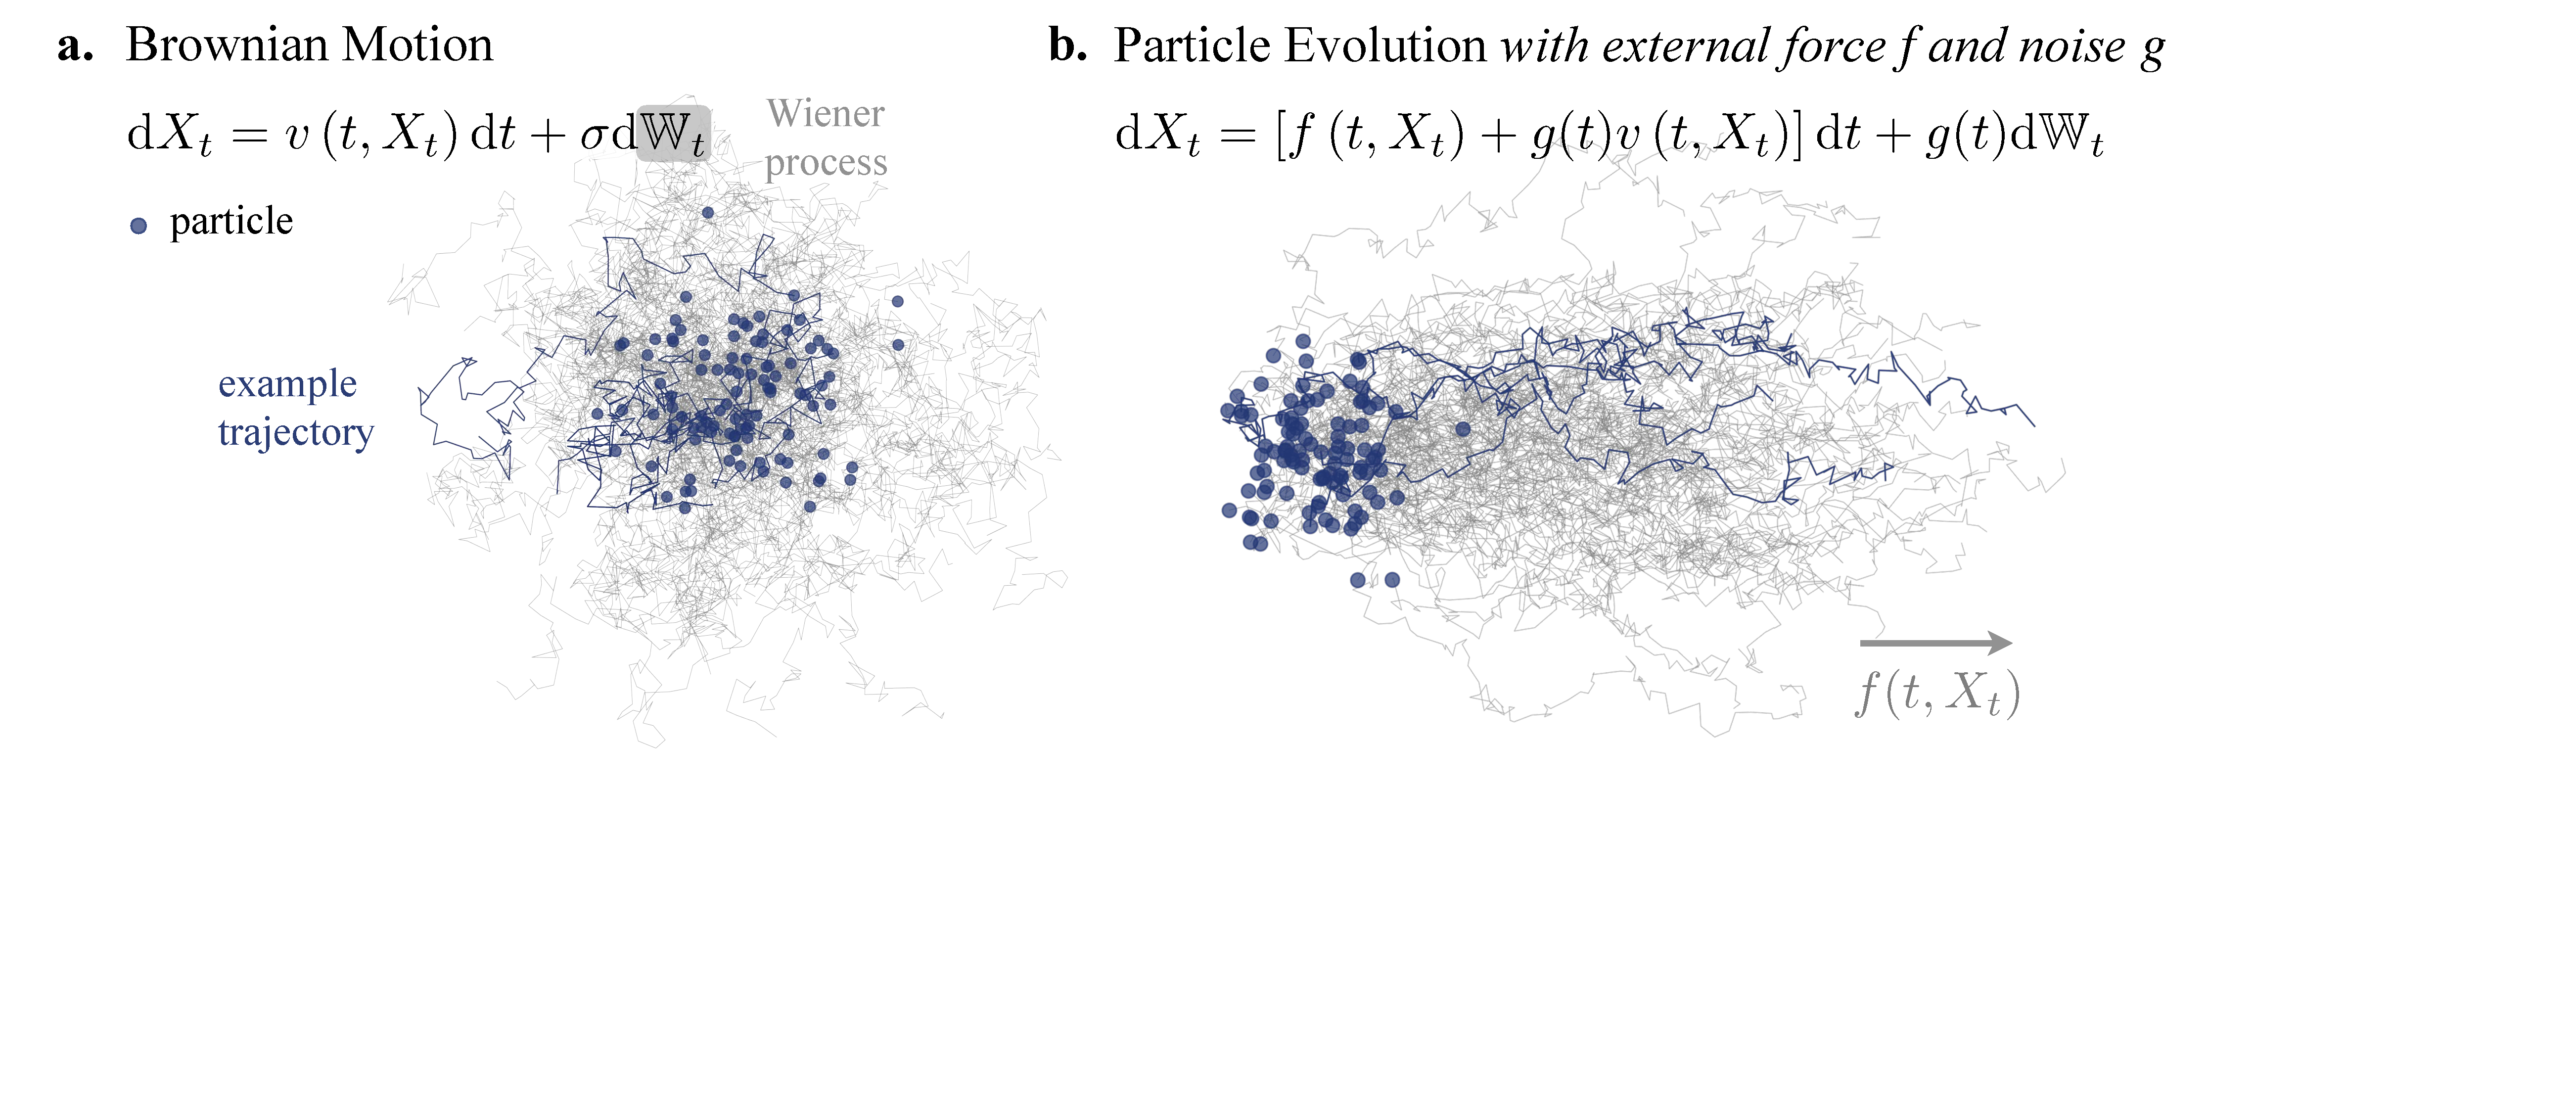
\includegraphics[width=\textwidth]{figures/fig_comparison_sdes.pdf}
  \caption{\textbf{Comparison of different SDE classes.} \textbf{a.} Particles evolve according to simple Brownian motion in all directions depending on the noise level $\sigma$. \textbf{b.} A particle evolution with an external speed $f$, here exemplified through a horizontal drift, and time-dependent noise $g$. The initial location of the particles is denoted as a blue dot, example trajectories are highlighted by blue lines.}	
  \label{fig:sde_comparison}
\end{figure}

\subsubsection*{Generalizations to Other SDE Classes}
To describe complex biological processes, however, we need to consider SDE classes comprising nonlinear drifts, affine control, and time-varying diffusion. 
In the following, let us consider SDEs with an external speed $f(\cdot, t): \mathbb{R}^d \rightarrow \mathbb{R}^d$, time-dependent diffusion $g(t) \in \mathbb{R}$, and standard Wiener process $\mathbb{W}_t \in \mathbb{R}^d$\footnote{Hereafter, we will sometimes drop $f \equiv f(t, X_t)$ and $g \equiv g(t)$ for brevity.}. \citet{caluya2021wasserstein, chen2021likelihood} provide a generalization of the above framework that reads
\begin{align}
\label{eq:sb_control_gen}
& \inf _{v \in \mathcal{V}} \mathbb{E}\left\{\int_0^1 \frac{1}{2}\norm{v(t, X_t)}^2 d t\right\}\\
\label{eq:sb_control_constraint_gen}
& \mathrm{d} X_t=\left[f\left(t, X_t\right)+g(t) v(t, X_t)\right] \mathrm{d} t+\sigma g(t) \mathrm{d} \mathbb{W}_t
 \\
\nonumber & X_0 \sim \mu_0, \quad X_1 \sim \mu_1,
\end{align}
with $g(t)$ being uniformly lower-bounded and $f(t, X_t)$ satisfying Lipschitz conditions with at most linear growth in $x$.
The effect of adding an external force $f$, here exemplified through a horizontal drift, compared to standard Brownian motion is visualized in \cref{fig:sde_comparison}.

\paragraph{Optimality criteria.}
Again, we recover the optimality criteria via a \citeauthor{hopf1950partial}-\citeauthor{cole1951quasi} transform  of \eqref{eq:sb_control_gen} resulting in
\begin{align} \label{eq:sb_optimality_gen}
& \frac{\partial \Phi}{\partial t}=-\nabla \Phi^{T } f- \frac{1}{2}\sigma^2 g^2 \Delta \Phi \quad \quad \text { s.t. } &\Phi(0, \cdot) \widehat{\Phi}(0,  \cdot)=\mu_0, \\
\nonumber & \frac{\partial \widehat{\Phi}}{\partial t}=-\nabla \cdot(\widehat{\Phi} f)+\frac{1}{2}\sigma^2 g^2 \Delta \widehat{\Phi} \quad &  \Phi(1, \cdot) \widehat{\Phi}(1, \cdot)=\mu_1
\end{align}
with the optimal control $v(t, X_t)= \sigma^2 g(t) \nabla \log \Phi\left(t, X_t\right)$.
The solution in \eqref{eq:sb_optimality_gen} can be expressed through two coupled SDEs of the form \citep{leonard2013survey}
\begin{align}
\label{eq:sb_forward} 
& \mathrm{d} X_t=\left[f+g^2 \nabla \log \Phi\left(t, X_t\right)\right] \mathrm{d} t+g \mathrm{~d} \mathbb{W}_t, \quad & X_0 \sim \mu_0, \\
\label{eq:sb_backward}
& \mathrm{d} X_t=\left[f-g^2 \nabla \log \widehat{\Phi}\left(t, X_t\right)\right] \mathrm{d} t+g \mathrm{~d} \mathbb{W}_t, \quad & X_T \sim \mu_T,
\end{align}
where $T = 1$, $\sigma = 1$, and $\nabla \log \Phi\left(t, X_t\right)$ and $\nabla \log \widehat{\Phi}\left(t, X_t\right)$ are the optimal forward and backward drifts for the \acrlong{SB}.

\looseness -1 Interestingly, the underlying SDEs  \eqref{eq:sb_control_constraint_gen} coincides with the dynamic systems considered in score-based generative models \citep{song2020score}, an emerging generative model class that has achieved remarkable results in synthesizing high-fidelity data \citep{song2019generative, kong2020diffwave}.
It also represents a key connection that has recently fueled the development of \acrlongpl{DSB} \citep{de2021diffusion, chen2021stochastic, bunne2022recovering, liu2022deep}, and will be subject of \cref{cha:neural_sde}.
Compared to classical diffusion-based generative models \citep{daniels2021score, song2020score}, these algorithms allow interpolation between complex distributions. Extended to the Riemannian geometry \citep{thornton2022riemannian, de2022riemannian}, it has found applications in molecular dynamics \citep{holdijk2022path, somnath2023aligned}, and cell differentiation processes \citep{vargas2021solving, bunne2022recovering, tong2023conditional}.
